\chapter{Methods}
\index{Methods@\emph{Methods}}%
\subsection{Estonian Phonetics}
The role of primary stress in Estonian is described by Ilse Lehiste as {\it identificational} rather than contrastive \citep{lehistePhoneticsMetrics1992}. In other words, there are no stress minimal pairs at the lexical level, so the prominence cue is to indicate the onset of a new word. This is sometimes also called {\it demarcative} stress.



Three proposed levels of stress: primary stress, unstress, and secondary stress. \citep{lippusAcousticStudyEstonian2014a}

Duration can be a phonetic correlate of stress, and it can also be independently contrastive at the segmental level \citep{lehistePhoneticsMetrics1992}. 
Primary lexical stress in native Estonian words is fixed, falling on word-initial syllables. 
\cite{eekmeisterUralica98}
\begin{exe}
\ex \gll laul-da \\
	{[ˈlɑuːl.dɑ]} \\
	sing-\Tr{} 
	\glt	`singing'
\ex 	ööbik \\
	{[ˈøː.pikː]} \\
	nightingale.\Nom{} 
	\glt`nightingale'
\end{exe}

Estonian has three syllable weights, also called degrees or quantities, that are contrastive in primary stress position. The first degree or Q1 is described as short, 
%In \ref{quant_cont}, we see two minimal pairs illustrating this contrast. 

This ternary contrast has long been the subject of debate in the phonological literature of metrics: Q3 syllables have been analyzed both as a monosyllabic foot \citep{princeMetricalTheoryEstonian1980} and as a trimoraic syllable \citep{hayesCompensatoryLengtheningMoraic1989, kuznetsovaEstonianWordProsody2018,prillopMoraeEstonianReply2020}. 


 \begin{table}[htb]
\centering
\begin{tabular}{lcc}
\hline

Q1 &		 sada 		& 	kabi  \\  
	&	 {\it `hundred'} 	&	 {\it`hoof' }\\
\hline
Q2 &		saada 		&	kapi \\
	&	 {\it`send' }		&	{\it`of the cupboard' }		\\
\hline
Q3 &		saada 	&	 kappi 	\\
	&	{\it`recieve' }	&	{\it`into the cupboard' }	\\
\hline
\end{tabular}
\label{qexamps}
\caption{ternary syllable weight contrast}
\end{table}



Acoustically, the difference between a stressed and an unstressed syllable is found not in a single cue but in a convergence of several cues: often duration, increased variability in f0, and increased vowel space, corresponding to a notion of localized hyperarticulation \citep{smiljanicProductionPerceptionClear2005, de1995supraglottal, lindblom1990}. 



\subsection{Estonian Phonetics}
The role of primary stress in Estonian is described by Ilse Lehiste as {\it identificational} rather than contrastive \citep{lehistePhoneticsMetrics1992}. In other words, there are no stress minimal pairs at the lexical level, so the prominence cue is to indicate the onset of a new word. This is sometimes also called {\it demarcative} stress.



Three proposed levels of stress: primary stress, unstress, and secondary stress. \citep{lippusAcousticStudyEstonian2014a}

Duration can be a phonetic correlate of stress, and it can also be independently contrastive at the segmental level \citep{lehistePhoneticsMetrics1992}. 
Primary lexical stress in native Estonian words is fixed, falling on word-initial syllables. 
\cite{eekmeisterUralica98}
\begin{exe}
\ex \gll laul-da \\
	{[ˈlɑuːl.dɑ]} \\
	sing-\Tr{} 
	\glt	`singing'
\ex 	ööbik \\
	{[ˈøː.pikː]} \\
	nightingale.\Nom{} 
	\glt`nightingale'
\end{exe}

Estonian has three syllable weights, also called degrees or quantities, that are contrastive in primary stress position. The first degree or Q1 is described as short, 
%In \ref{quant_cont}, we see two minimal pairs illustrating this contrast. 

This ternary contrast has long been the subject of debate in the phonological literature of metrics: Q3 syllables have been analyzed both as a monosyllabic foot \citep{princeMetricalTheoryEstonian1980} and as a trimoraic syllable \citep{hayesCompensatoryLengtheningMoraic1989, kuznetsovaEstonianWordProsody2018,prillopMoraeEstonianReply2020}. 


 \begin{table}[htb]
\centering
\begin{tabular}{lcc}
\hline

Q1 &		 sada 		& 	kabi  \\  
	&	 {\it `hundred'} 	&	 {\it`hoof' }\\
\hline
Q2 &		saada 		&	kapi \\
	&	 {\it`send' }		&	{\it`of the cupboard' }		\\
\hline
Q3 &		saada 	&	 kappi 	\\
	&	{\it`recieve' }	&	{\it`into the cupboard' }	\\
\hline
\end{tabular}
\label{qexamps}
\caption{ternary syllable weight contrast}
\end{table}



Acoustically, the difference between a stressed and an unstressed syllable is found not in a single cue but in a convergence of several cues: often duration, increased variability in f0, and increased vowel space, corresponding to a notion of localized hyperarticulation \citep{smiljanicProductionPerceptionClear2005, de1995supraglottal, lindblom1990}. 




I first describe the source materials and the selection criteria for the sample corpus of {\it regilaul} folksongs. Following this, the annotation and measurement procedure is detailed. Then the procedure for assembling the corpus of songs and their text annotations is covered before proceeding to the inclusion criteria for vowel duration and dispersion measurements.


\section{Design of the Present Study}

autosegmental and segmental tiers

\subsection{Long Vowels and Diphthongs}
CV vs segmental dichotomy of CV phonology, as reflected in the suprasegmental aspects of vowels. 

An estonian word game supports the notion of many-to-one phonemes for long vowels, but a one-to-one status for diphthongs.



\begin{exe}

\ex  long vowels (Q1,Q2, Q3 contrast) 
	\begin{itemize} 
	\item sada `hundred' $\rightarrow$ sapida 
	\item  saada `send' (2nd sg. imp.) $\rightarrow$ sapiida (*sapiada)(*saapida)
	\item saada `get' , {\it -da} infinitive $\rightarrow$ sapii:da (*sapiada)(*saapida)
	\end{itemize}
\ex 	 diphthongs \\
laulus `in the song' (iness.sg) $\rightarrow$ lapiulus (*laupilus)
\end{exe}

In both cases, `pi' carries the prosodic characteristics of the displaced syllable. the stress is moved from first syllable to 'pi,' and also the length. crucially, the diphthong is split at the segmental level, while the long vowels are not. 

long vowels are treated as monophonematic, whereas diphthongs are treated as biphonematic. 

\cite{lehiste85, vago85}

As previous studies found that the durational properties of quantity contrasts were not found at the level of the syllable or the foot, I investigate the fine-grained acoustic-phonetic properties of these contrasts at the segmental level within the syllable-note of the song. 


To investigate the acoustic manifestations of stressed and unstressed syllables in {\it regilaul}, syllable nuclei from disyllabic feet in Q1 and Q2 are compared, as Q3 never appears in unstressed positions. 
%
%Q1	CV 		CVC
%Q2 	CVV		CVVC 	CVCC

The syllables are further compared by position in the song according to the beat: 

To investigate the question of quantity opposition in {\it regilaul}, disyllabic feet in Q1, Q2, and Q3 are examined according to their relationship to the beat. 



\subsection{segmentation criteria}

no syllables in verse-final or musical phrase-final position
vowel onset:
if sonorant onset, when intensity within 2 dB of steady-state/medial position of the vowel and intensity slope approaching zero
or the intensity slope approaching zero (less than or equal to one) for more drastic transitions such as obstruents
vowel offset intensity: before slope exceeds one (less than or equal to one) in transition to occlusion

primarily syllables with onsets

adjacent vowels across word boundaries, a glottal stop if present in the acoustic signal, otherwise omitted

lateral approximants in syllable onset usually easier to determine boundary, coda position /l/ no boundary definable and thus analyzed as a diphthong
in the case of intersyllabic long /l/, however, as there is no way to determine the end of the coda /l/ and beginning of the onset /l/, are excluded

song 41 contained churchbells
cases wherein word boundaries unclear due to transcription of the lyrics/poetic license

nonsense words

epenthesized vowels (i.e., pandi mind paju raiumaie) having mind(e) \\
word-final vowel next to word-initial vowel/difficult or impossible to determine end of preceding and onset of next across word boundaries


vowel onset and offset boundaries were determined using chiefly pitch and intensity contours in addition to the three first formants.



onsets: \\

plosive: not include burst. three first formants visible. slope of pitch and intensity contours encroaching on the respective steady state, with a slope less than or equal to one. 

liquids: formant steady state, steady pitch and steady intensity. 

nasals: intensity at least half of level within following vowel, antiformants, steady f0. intensity reduces in vowels. 

fricatives: following the end of the visible noise in the spectrum, at the point where intensity and formant contours are both visible and steady. The /s/  have reliable pitch carats immediately preceding vowels. \ref{spitch}. 

codas: \\

plosives: preceding fall in f0 and intensity
allow for more variation in formants of codas, other cues more consistent.

nasals: drop in f0, intensity less than half of the way to the level within-vowel. 

liquids: before drop in intensity 
before formant divergence.

across syllable and word boundaries: \\

adjacent vowels, when possible, segmented by presence of glotallization pulses and categorical changes in pitch. \\

In all cases, if the aforementioned cues are unavailable or ambiguous, the token is elided for this analysis. \\

A total of 757 individual vowel nuclei met the criteria for inclusion in duration measurements. After excluding diphthongs, a subset of _ met the criteria for inclusion in vowel space measurements. 


\subsection{Vowel Duration}
Why vowels and not entire syllables? The reason for this is twofold. First, measuring only the syllable nuclei affords more accurate automation. Were we to measure entire syllables, we would be limited to those with sonorant onset consonants, or in a restricted set of environments where consonant onset would be definable. By measuring only the syllable nuclei, we can reliably include more of the available vowel instances. Second, using the sonorant portions of the syllables makes way for the use of onset detection algorithms, so a strong beat is defined by a consistent threshold for each song, relative to the strength of the other beats in the signal. \\
The previous regilaul studies found evidence of syllable-note isochrony. So, if we see Q2 and Q3 vowels increasing in duration, this would be evidence against those findings. If, however, the long and overlong vowels have less duration than the short ones, this is evidence supporting syllable-note isochrony. Due to the structure of heavy syllables, the vowels must shorten in order to accommodate the additional coda segments within the note. 


\subsection{Vowel Space Area and Dispersion}

As a second measure of prominence, we include vowel space area and dispersion. Studies in English have shown that stress can be thought of as localized hyperarticulation or clear speech. \cite{deJong} Vowel space area and dispersion are well documented acoustic correlates of clear speech in English \cite{bradlow}, and has also been confirmed in cross-linguistic studies with Croatian \cite{rajka} and others. \\

While it has not yet been documented as an acoustic correlate of stress in Estonian, I have reason to believe that it will be an available cue for a singer to use, especially in the context of a song. While duration may or may not be an available prominence cue at the word level, vowel space area and dispersion are prominence cues that would not conflict with the prosodic hierarchy of the song. 

often, resonators or filters of musical instruments are solid or fixed. This is not the case with the vocal instrument.



then so long as the word-level categories of quality are preserved, the 


\section{Materials}

\begin{figure}[htbp]
\centering

\includegraphics[width=300pt]{figures/055.png}
\caption{Laula! {\it Sing!}}
\label{default}
\end{figure}




The data for this study was sourced at the Estonian Folklore Archives (EFA). 
\citep{orasEstonianFolkloreArchives2022a}.



Until 1948, songs were collected on wax cylinders, then played on a phonograph and transcribed. shellac discs 1936-38, 746 recordings, 
analogue is the biggest collection in the archive, with over 80,000 individual recordings. Open-reel tape, cassette recordings since the 1970s. 
both wax and disc were re-recorded onto open-reel tape in 78-79.
Presently, the sound engineer Jaan Tamm has been working on preserving the earlier tape recordings in digital form for the EFA. WAV files are stored on CD-Rom at the EFA in Tartu, Estonia, while .mp3 and .ogg lossy formats are uploaded to the internet database. 
% collected by Herbert Tampere, Erna Tampere, and Ottilie Kõiva between 1912 and 1966 for the Estonian Folklore Archives in Tartu, Estonia. \\
%
% and   tunes
%the total number of song recordings is over 26,000. Of these, over 11,000 are from the beginning of the 20th century. Tampere did like 2,000 of them..
%
%%
%The need for writing the tunes live during fieldwork has reduced with the availability of analog and now digital audio recording equipment.




Songs for this paper were accessed via The Anthology of Estonian Traditional Music \citep{tampereAnthologyEstonianTraditional2016}. Originally published on four vinyl discs in 1970(\ref{vinyl1970}, the digital version showcases a robust sample of the massive collection of {\it regilaul} in Estonian Folklore Archives. In addition to audio, the  compilation includes  photographs, sheet music, and performer demographics of 98 {\it regilaul} songs and 17 instrumental tunes. 
These songs were compiled in part by Herbert Tampere, an early ethnomusicology field work organizer of the EFA, who along with Erna Tampere and Ottilie Kõiva collected these folk songs. Pictured in \ref{tampy} is a photograph taken of one of the very field trips to record songs studied in this paper. 

\begin{figure}[htb]
\centering

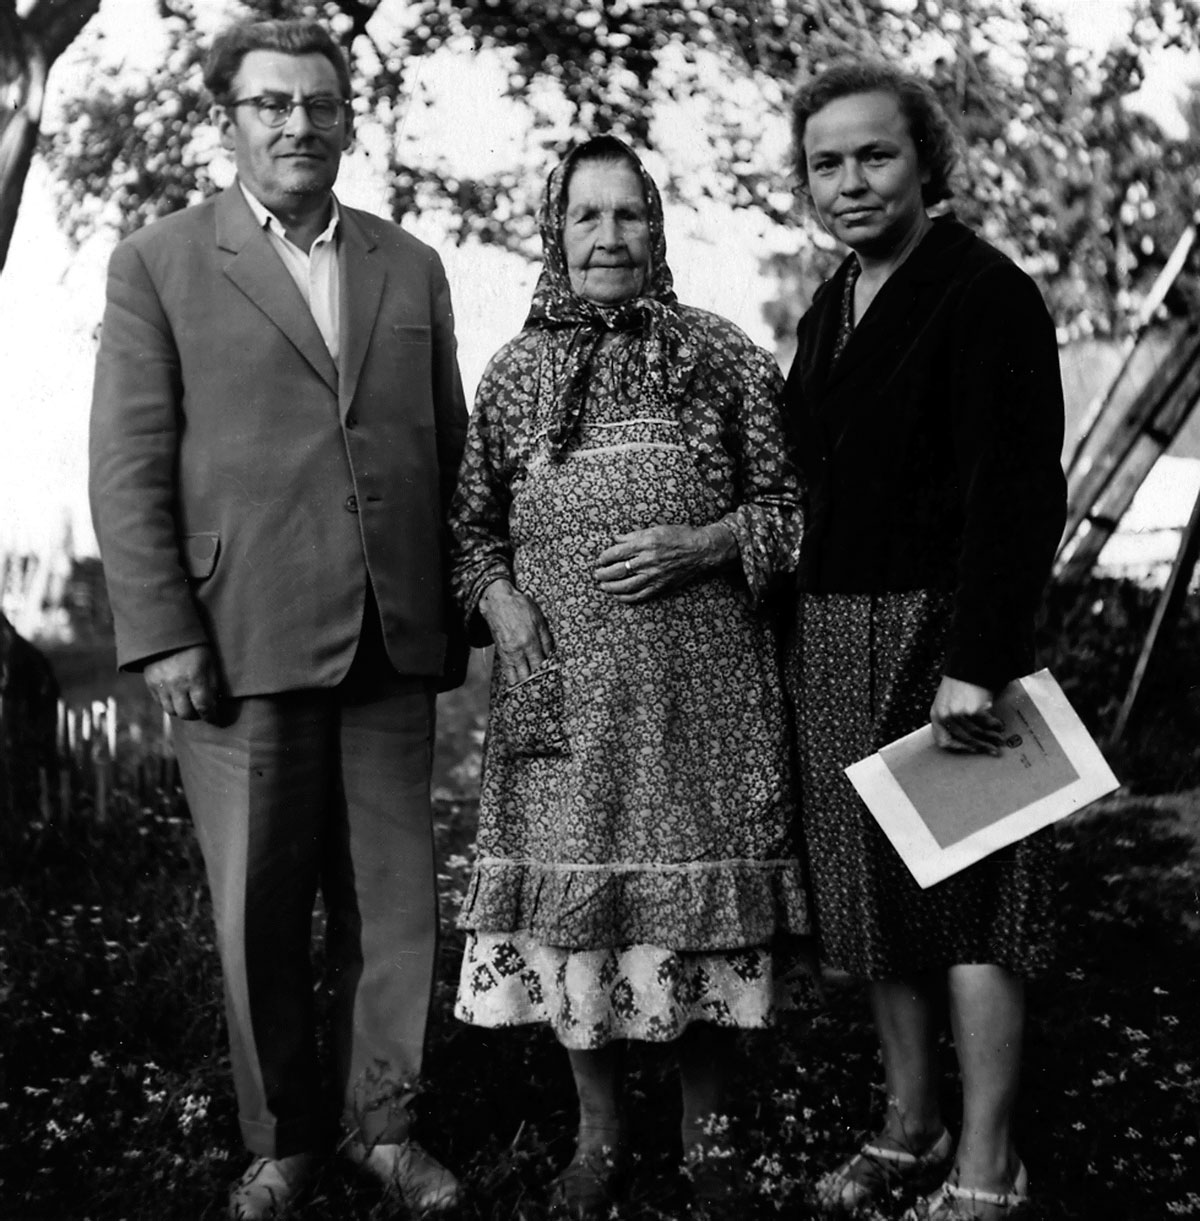
\includegraphics[width=200pt]{figures/Mf_07027_Tampered_Orik.jpg}
\caption{Herbert Tampere on a field trip}
\label{tampy}
\end{figure}


While the ultimate goal is to continue annotation of the entire available corpus of {\it regilaul}, for the initial analysis I chose a sample of songs all belonging to the same regional dialect and recording method. Once several regions were identified as possible candidates, a native Estonian speaker was consulted on the final selection. The nine songs analyzed in this study were all recorded in Parnümaa county from 1961-1966 by Herbert and Erna Tampere. 
% The first criteria is due to the lossy nature of some of the older files available on the site: the online versions are all compressed lossy, so the analog audio originally recorded on tape and then digitized have a higher resolution, even compressed, than songs that have been copied from wax cylinders or shellac discs onto open-reel tape and then digitizing. 


\section{Annotating the Song Audio }



 Each song's lyrics are copied from the site and saved as .txt files in Estonian orthography, each line of the file corresponding to one melody line.  
Audio files of the selected songs are downloaded from the archive in .ogg format, which is the highest resolution of the two lossy\footnote{define lossy} formats available from the digital anthology. Each song is then imported into a Logic Pro X \citep{b131156} session for beat detection, tempo mapping, and trimming. 
To make the tempo map, the session must be set to {\it flex tempo}. From here a beat onset detection algorithm \citep{robertsonBKeeperBeattrackerLive2007} is  given the transcribed bpm and time signature from the archived song data and run on the imported audio file. The result is an annotation of intervals in time, and the bpm for each measure is annotated according to the performance of the song.
The tempo map allows us to document when {\it exactly} in time the particular singer performed a given note, the duration of the sung note, and the acoustic threshold by which the note is defined as ``strong" relative to surrounding notes. The process is informed by the transcribed bpm and time signature included in the anthology. This is beneficial to my purposes in two ways: by accounting for the natural tempo variation in live performance, and by using a consistent metric to determine beat strength acoustically rather than just perceptually.

 From here, a MIDI track is programmed to create a metronome that is the length of a single syllable-note in the song. In most of these, a 4/4 measure contains eight eighth notes, so the metronome track contains four eighth notes indicating the ``ictus" beats. In flex tempo mode, the MIDI track adjusts note and measure length to match the fluctuations in tempo as documented in the map for the song. The metronome and the song audio file are trimmed to match exactly, and the metronome is converted into a textgrid in PRAAT\citep{boersnaPraatDoingPhonetics2022}, where the annotation process continues. 

 


The orthographic text phrases of the song lyrics are then inserted into each phrase interval with a script, and then eSpeak forced aligner for Estonian \citep{duddingtonESpeakSpeechSynthesizer1995} is run on each phrase to the word and phonemic level. Because this forced aligner is trained on spoken, not sung Estonian, the aligner sometimes tries to align words into the signal before they are uttered. In these cases, the word level tier is manually realigned so that it contains all and only the transcribed word, and then the forced aligner is re-run on this word to the segmental level. In the case of a vowel interval containing an obvious silent portion or occlusion, the boundary is manually adjusted to only include sonorant portions of the signal. 
% \begin{figure}[ht]
%\begin{center}
%			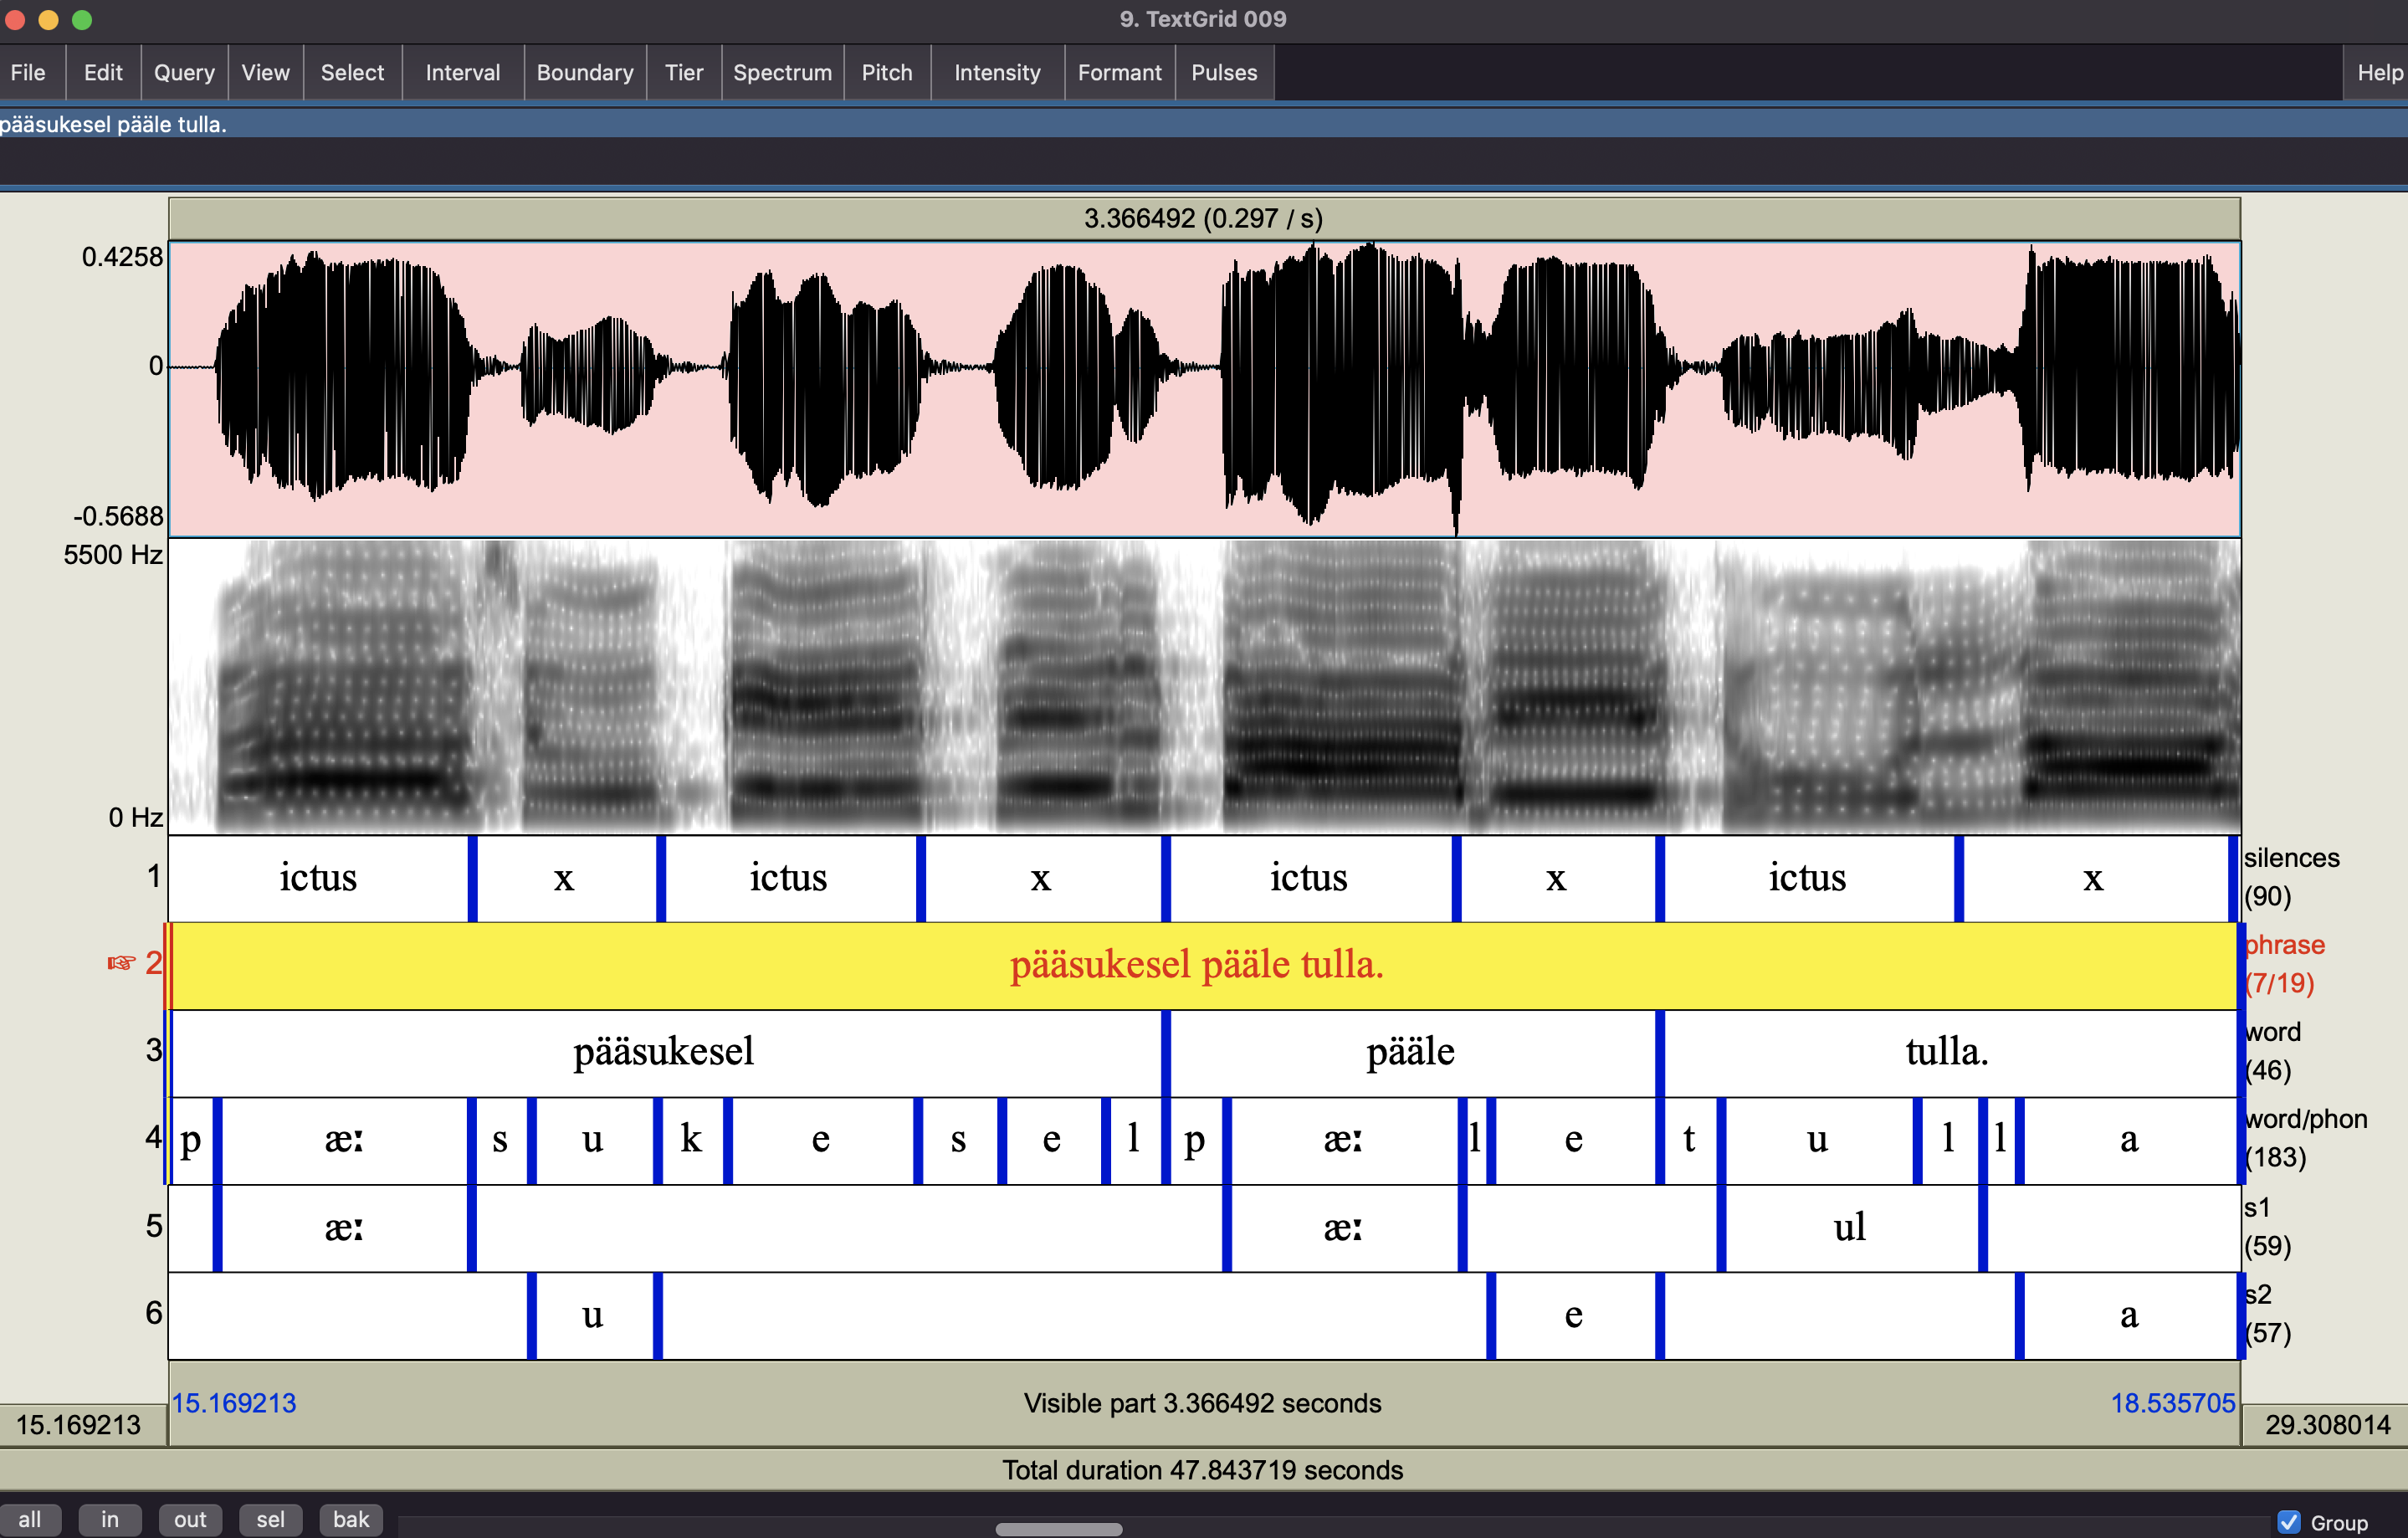
\includegraphics[width=300pt]{figures/phrase_grid.png}
%			\caption{single phrase annotation}
%\label{phrase}
%\end{center}
%\end{figure}
%\begin{figure}[hb]
%		\begin{center}
%			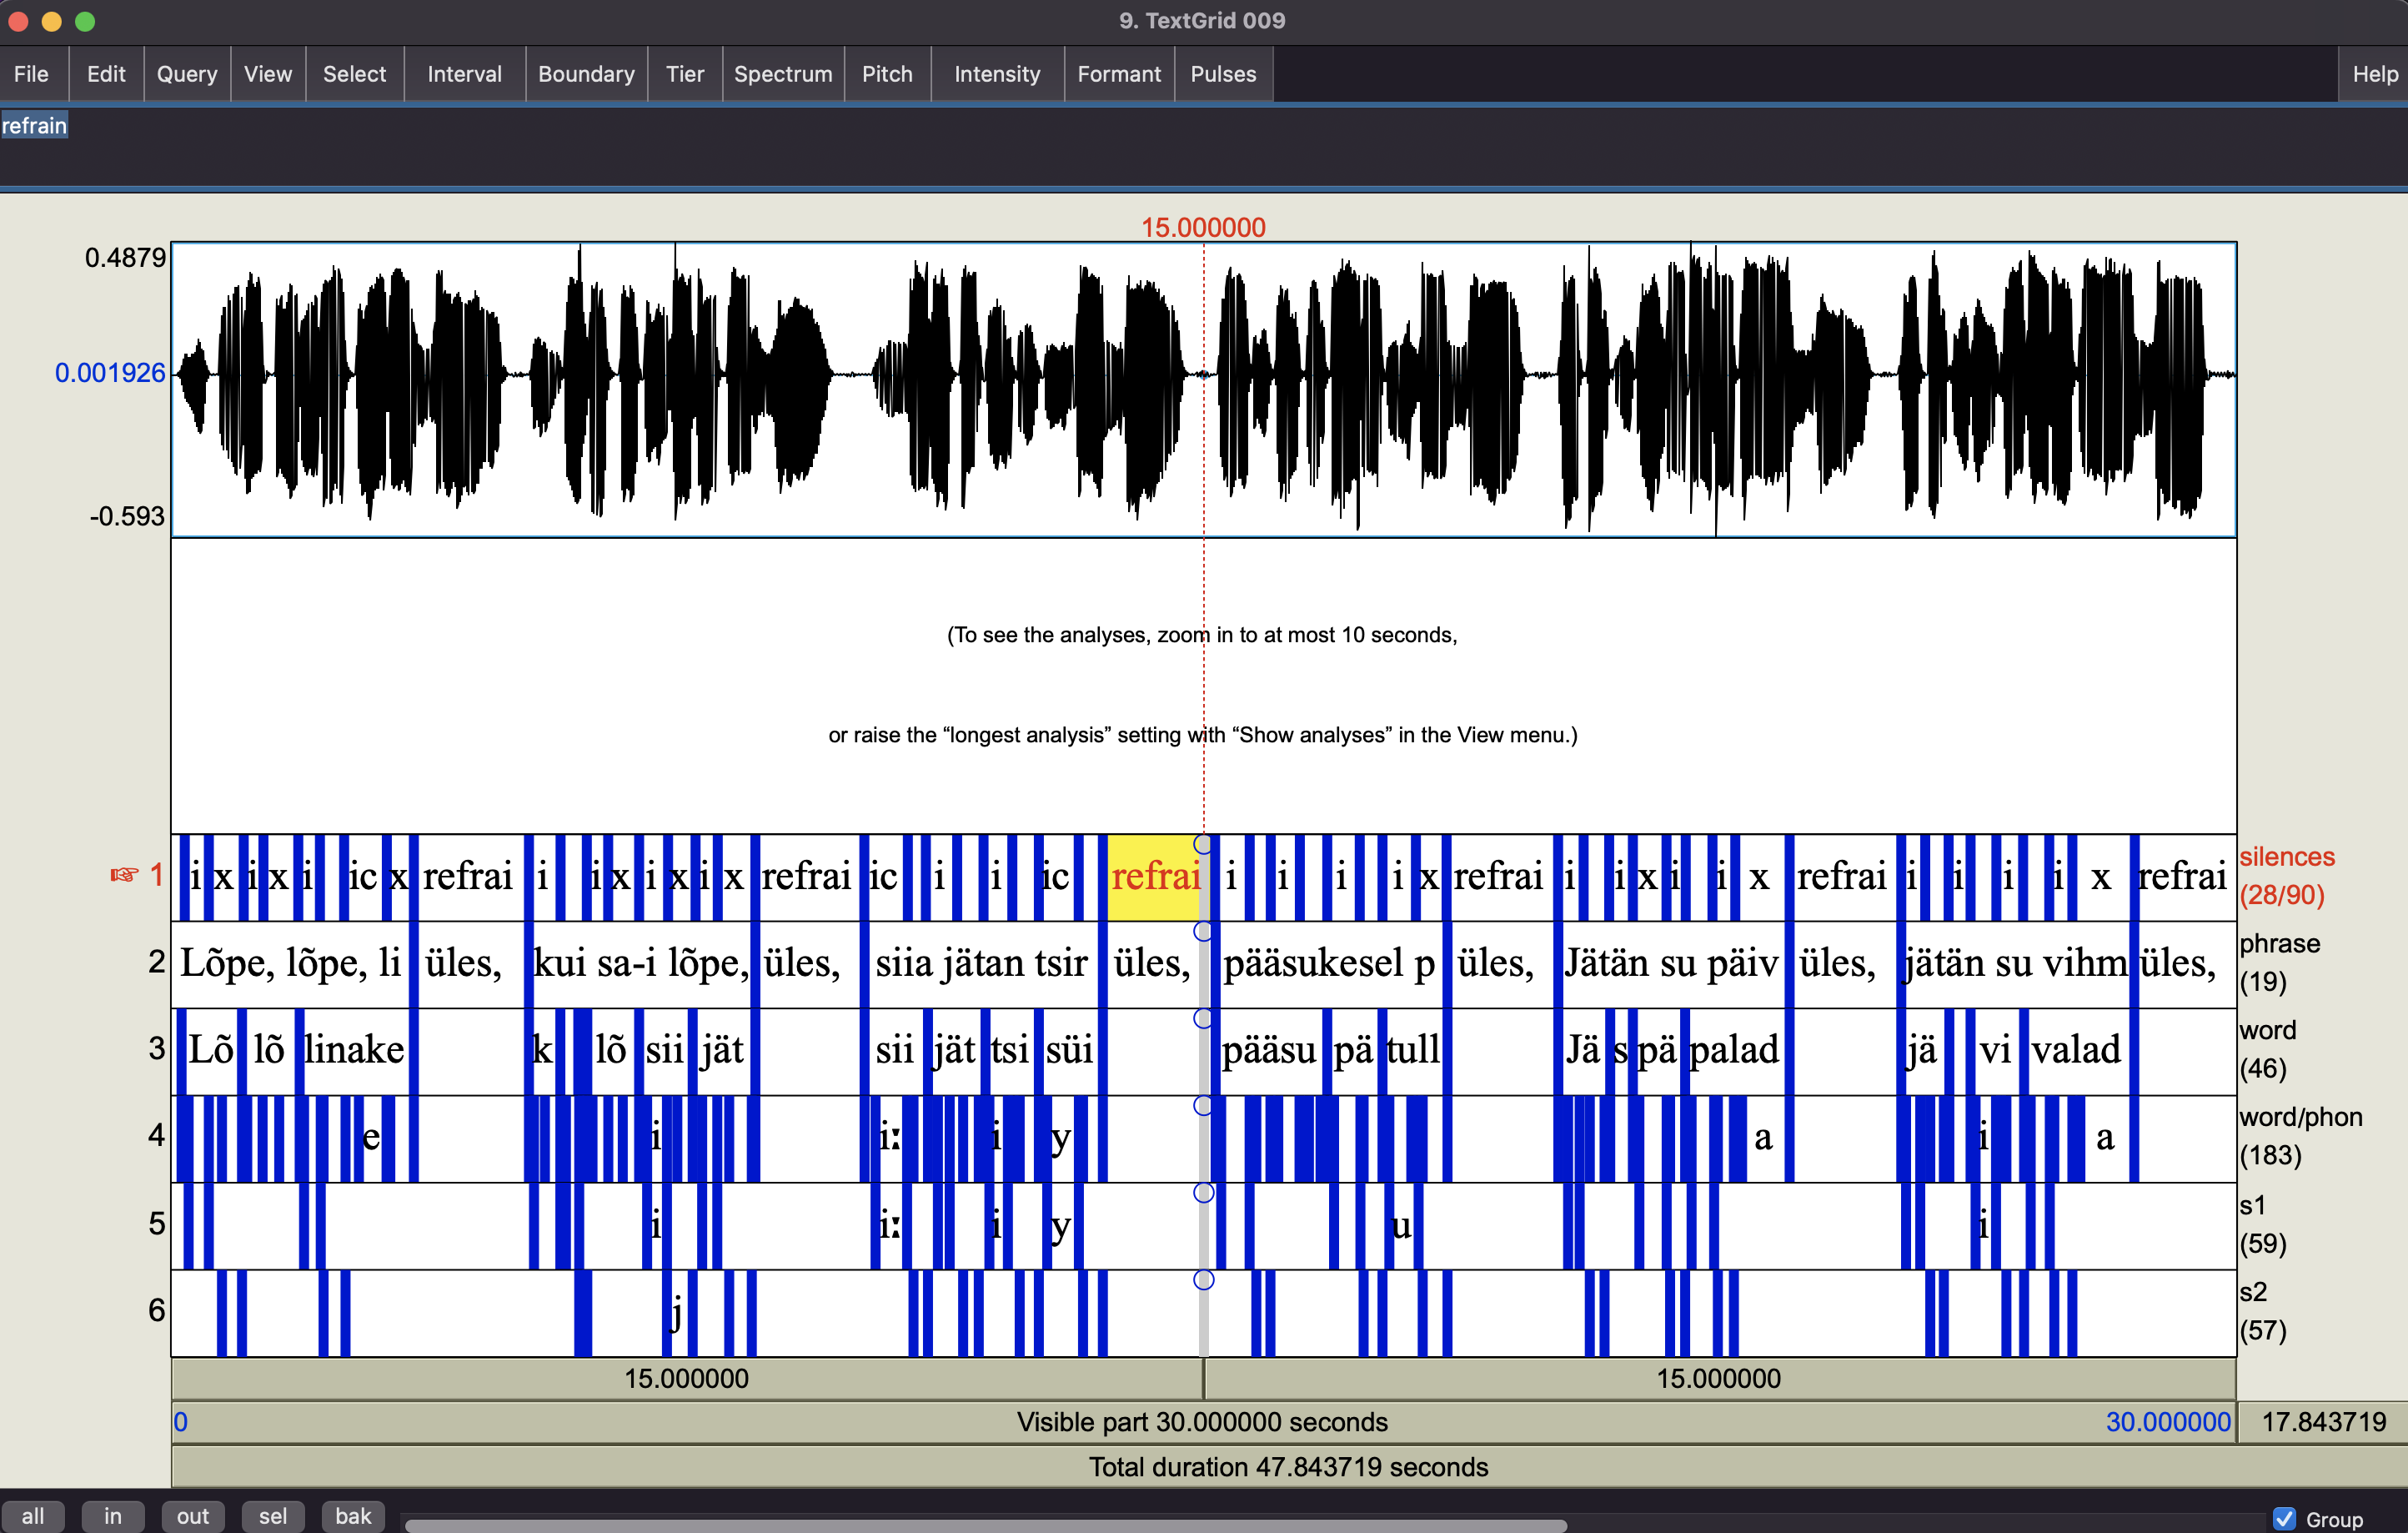
\includegraphics[width=300pt]{figures/big_grid.png}
%			
%			\caption{whole song annotation}
%			\label{songwhole}
%		\end{center}
%\end{figure}
%	
%	 In \ref{phrase} is a completed annotation of a single phrase from a song, and in \ref{songwhole} is an entire song file's interval annotation.

At this point, the audio recording of each song has tiers annotated for tempo and strong beat, verse line phrases, two interval tiers force-aligned to word and phoneme levels, and a separate tier with intervals of the individual vowel segments of interest copied from the phoneme tier.
\section{Assembling the corpus and annotations}
The last step in preprocessing is to integrate the annotation of the song audio with the lexical content of the song. This study accomplishes the task using an open-source natural language toolkit in python called estinltk \url{https://github.com/estnltk} \citep{laur-EtAl:2020:LREC}. Among other things, the toolkit has a robust dictionary of Estonian grammar, including phonetic transcription of syllables with quantity and stress data. 


Thus the data structure of this corpus offers two independent metrics of rhythmic prominence in these songs. From the audio recording and the beat detection, we have an annotation of strong beats based on replicable acoustic measurements, and from the dictionary in the natural language toolkit, we have native speaker intuitions about the lexical weight and prominence in the words of the text. While the stress system is generally predictable, the syllable quantity is not always apparent from the orthography, and not always detectible by a non-native listener. Linguistic descriptions of the Estonian language date back as early as the seventeenth century, but the ternary quantity contrast was not documented until native Estonian linguists contributed their intuitions. The non-native linguists had only described lexical stress \citep{sargEarlyHistoryEstonian2005a}. \\

Using onset detection algorithms such as these \citep{robertsonBKeeperBeattrackerLive2007} in phonetics research, especially in the interdisciplinary field of linguistics and musicology, will be particularly beneficial to answering questions about rhythm: finding a way to bring our intuitions and impressions about ``the beat" together with the acoustic phenomenon. By automating the annotation and measurement process using open source tools, the author hopes to share these machines with those who have similar research interests, and also to invite contributors to the data of this corpus of text data time-aligned to queryable audio signal data. 

\section{Study Design}
\subsection{Questions and Hypotheses}

\subsection{Inclusion Criteria for Vowel Measurements}

Once the annotations are complete, the corresponding text files are aggregated and, the corresponding measurements from PRAAT are concatenated via python using the parselmouth library python interface to PRAAT \citep{parselmouth, van1995python}. 
 I extracted vowel intervals which met the following inclusion criteria. For this study, we are interested in the durations of vowels in initial and pen-initial syllable-notes that are transcribed as isochronous in the melodic transcription. 

\subsection{Statistical Analysis} 
Linear mixed-effects model using lme4 in R \cite{rlme4}. 

For stress and ictus, only q1 and q2 syllables (Q3 never unstressed). \\
for quantity and ictus, only word-level stressed syllables



Design-based formula
Hierarchical Linear Model with group-specific terms

\cite{goodrichRstanarmBayesianApplied2020,brillemanJointLongitudinalTimetoevent2018}
